\documentclass[a4paper]{article}

\usepackage[a4paper,left=3in, right=1in]{geometry}
\usepackage{graphicx}
\usepackage{tikz}
\usepackage{xcolor}

\setlength{\parindent}{0pt}
\pagestyle{empty}
\pagecolor[HTML]{FFF0C9}

\usepackage{xepersian}
\settextfont{IRNazanin}[
  Extension=.ttf,
  BoldFont=*Bold,
  ItalicFont=*Italic,
  BoldItalicFont=*Bold,
  Path=fonts/
]

\begin{document}

\begin{tikzpicture}[remember picture, overlay]
  \node[anchor=north west, rotate=-40] at ([xshift=2cm,yshift=4cm]current page.north west) 
    {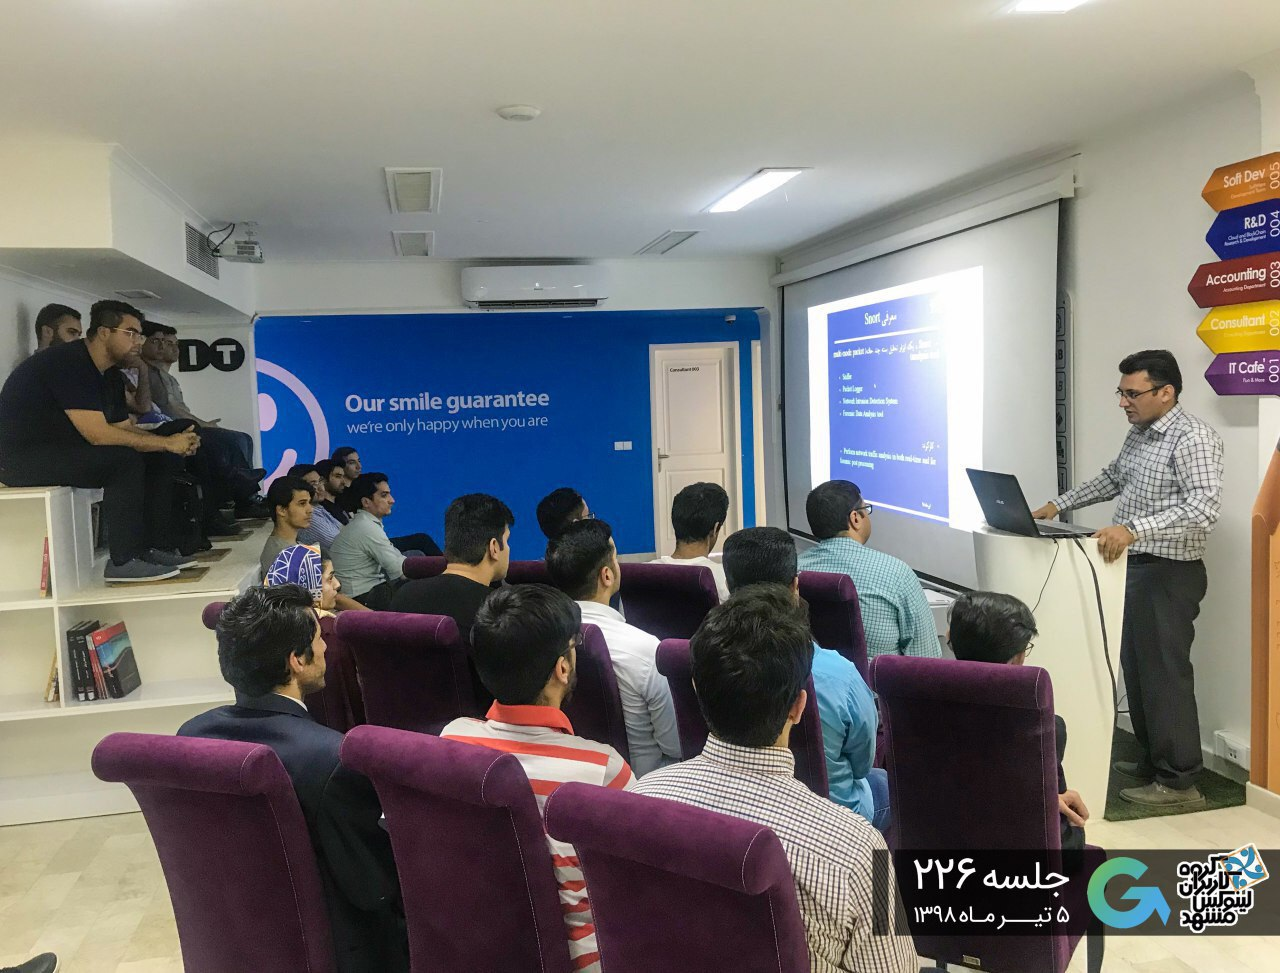
\includegraphics[width=0.50\paperwidth]{assets/session1.jpg}};

  \node[anchor=west, rotate=8] at ([xshift=-3cm]current page.west)
    {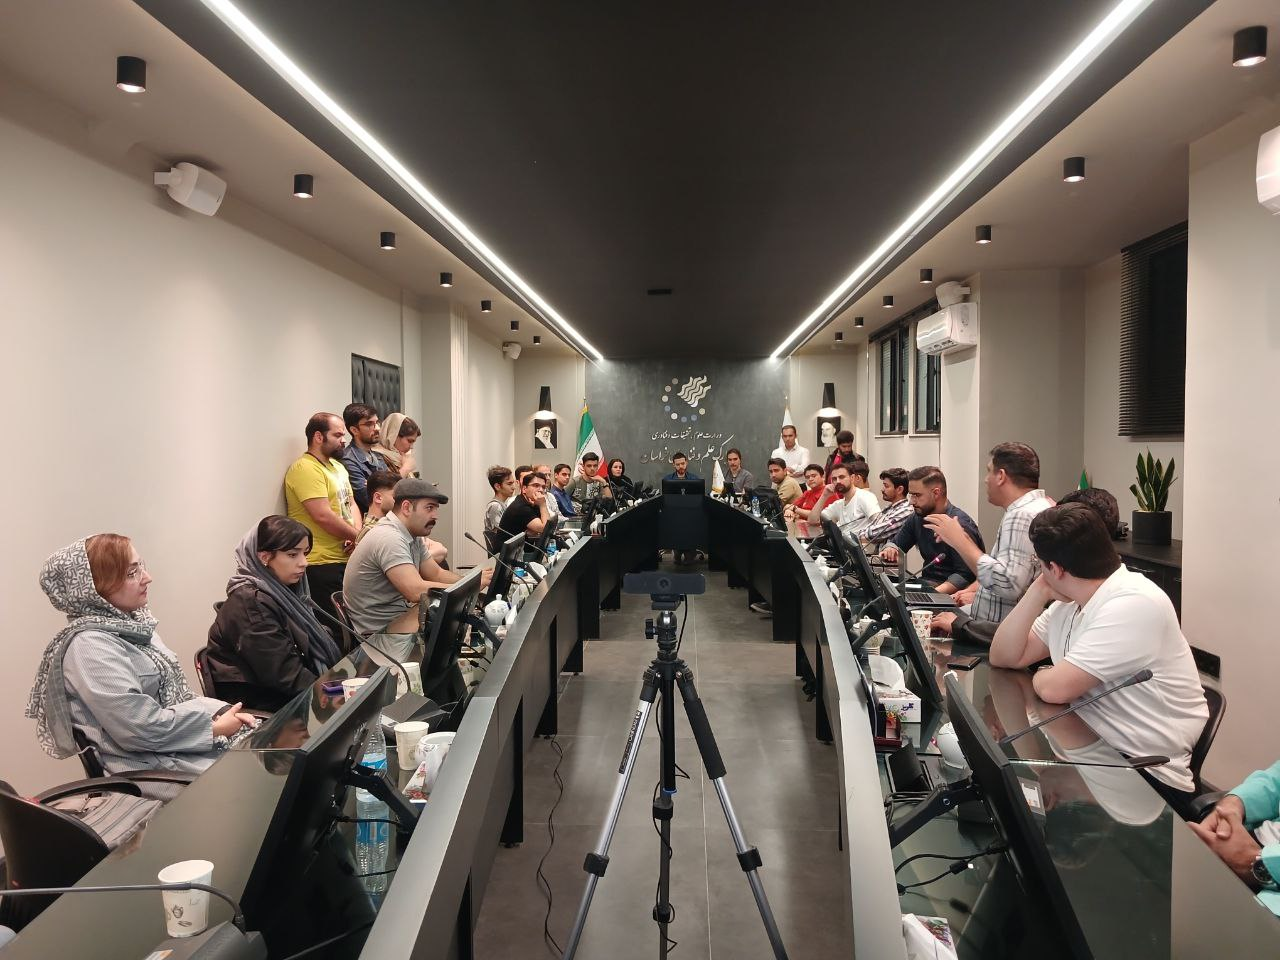
\includegraphics[width=0.40\paperwidth]{assets/session2.jpg}};

  \node[anchor=south west, rotate=40] at ([xshift=2cm, yshift=-5cm]current page.south west)
    {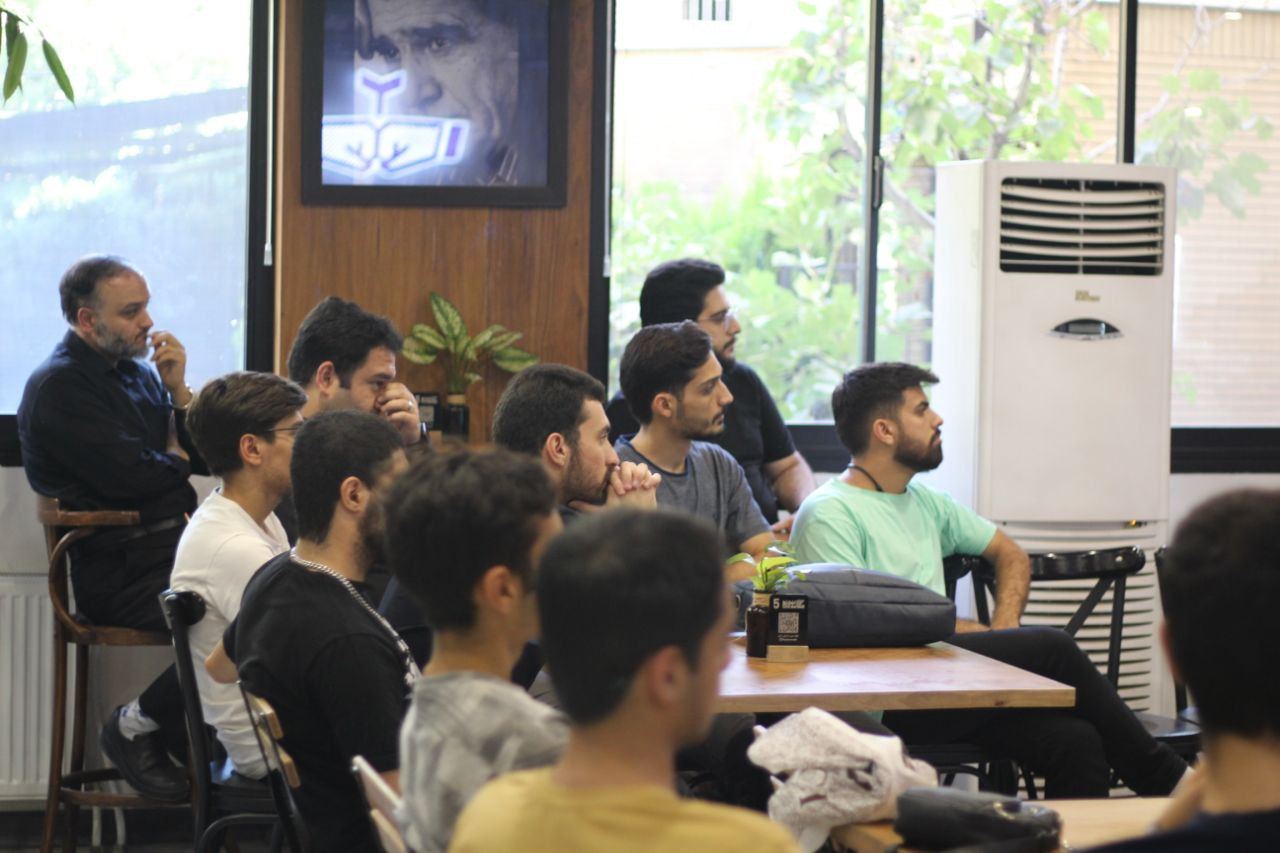
\includegraphics[width=0.65\paperwidth]{assets/session3.jpg}};

  \node[anchor=south east] at ([xshift=-1cm, yshift=1cm]current page.south east)
    {
\includegraphics[width=4cm]{assets/qrcode.png}};
\end{tikzpicture}


\begin{minipage}{0.2\textwidth}
  
\includegraphics[width=2cm]{assets/logo.png}
\end{minipage}
\hfill
\begin{minipage}{0.7\textwidth}
  \raggedleft
  {\Huge مشهدلاگ}\\\vspace{0.2cm}
  {\Large \lr{Mashhad LUG}}
\end{minipage}

\vspace{1cm}

گروه کاربران لینوکس مشهد (مشهدلاگ) یک سازمان غیرانتفاعی است که از سال ۱۳۸۶ تا امروز با برگزاری بیش از ۲۸۰ رویداد فنی، جامعه‌ای فعال از علاقه‌مندان به نرم‌افزار آزاد و فناوری‌های متن‌باز را در کنار هم گرد آورده است.

اهداف ما از روز نخست تا امروز ثابت مانده‌اند:

\begin{itemize}
\item ترویج و حمایت از سیستم‌عامل گنو/لینوکس و نرم‌افزار آزاد
\item آموزش فناوری‌های روز متن‌باز و مفاهیم پایه‌ی گنو/لینوکس
\item گردآوری و پیوند میان علاقه‌مندان و متخصصان این حوزه
\end{itemize}

فعالیت‌های مشهدلاگ تنها محدود به ارائه‌های فنی نیست؛ ما تلاش می‌کنیم جامعه‌ای پویا بسازیم که از کاربران تازه‌کار تا متخصصان باتجربه را دربرگیرد.
انواع رویدادهایی که تاکنون برگزار کرده‌ایم عبارتند از:

\begin{itemize}
\item ارائه‌ها و نشست‌های فنی
\item کارگاه‌های آموزشی
\item جشن‌های نصب و معرفی لینوکس
\item نشست‌های آزاد برای گفت‌وگو و تبادل تجربه
\end{itemize}

در طی سال‌ها، سازمان‌ها و شرکت‌های بسیاری از فعالیت‌های ما حمایت کرده‌اند و مشهدلاگ را بستری ارزشمند برای رشد جامعه‌ی فناوری مشهد دانسته‌اند.
از جمله حامیان سال‌های گذشته می‌توان به گرین‌وب، دانشگاه فردوسی مشهد، فاوا رضوی و دیگر اسپانسرهای گرامی اشاره کرد.

چرا از مشهدلاگ حمایت کنید؟

با حمایت از مشهدلاگ، شما مستقیماً به رشد و پویایی جامعه‌ی متن‌باز کشور کمک می‌کنید و در کنار آن، برند خود را در میان هزاران توسعه‌دهنده، دانشجو، و متخصص فناوری مطرح می‌سازید.

حمایت شما می‌تواند در قالب‌های زیر باشد:

\begin{itemize}
\item حمایت مالی از برگزاری نشست‌ها و کارگاه‌ها
\item پشتیبانی تجهیزاتی یا ارائه‌ی فضا برای برگزاری رویداد
\item معرفی فرصت‌های شغلی و همکاری به اعضای جامعه
\end{itemize}

ما باور داریم که رشد نرم‌افزار آزاد بدون همراهی جامعه‌ی حرفه‌ای و کسب‌وکارهای نوآور ممکن نیست.
از شما دعوت می‌کنیم تا در کنار ما باشید و در گسترش این مسیر نقش داشته باشید.

\end{document}
